\subsection{Architecture Verification}

%AGREE analysis of RTA arch in AADL

One of the steps for design-time assurance of the RTA architecture is verifying the architecture satisfies its high-level requirements.  Traditionally, requirements verification has been achieved using a combination of directed testing methods and manual review. However, model-based specification enables a more rigorous approach to verification via formal methods analysis. With both the requirements and architecture represented in formal (well-defined, unambiguous) notations, satisfiability modulo theories (SMT) solvers can be employed to determine whether there is any possible sequence of inputs that will violate a requirement.  Furthermore, failure by the solver to find a counterexample is essentially equivalent to a mathematical proof that the requirement can never be violated.  

In architectural models, we can represent high-level requirements as assume-guarantee contracts on components.  \textit{Guarantees} are statements about a component's outputs which will always hold as long as stated \textit{assumptions} are valid.  When designing an architecture that includes multiple components, it is imperative to verify that a system's subcomponent contracts satisfy the overall system contract, as well as whether a component's assumptions are valid with respect to the specified upstream guarantees and the environment.
%
We use the Assume Guarantee Reasoning Environment (AGREE)~\cite{agree2012} to specify and analyze component contracts in our run-time assurance architecture.  AGREE is a plugin for the Open Source AADL Tool Environment (OSATE), enabling contracts to be specified directly on AADL model components and analyzed within the modeling environment.

%The RTA architecture was modeled in AADL (Figure~\ref{fig:rta-agree}) using the Open Source AADL Tool Environment (OSATE), and the high-level requirements were added to this AADL model as AGREE specifications \cite{agree2012}.  AGREE specifications are used to describe component behavior through assume-guaranteee contracts, and these contracts are analyzed using AGREE's compositional reasoning framework available through the AGREE plugin for OSATE.

The main objective of our AGREE analysis of the collision avoidance system was to verify that the RTA architecture is guaranteed to publish only safe flight plans.
%
%In Figure~\ref{fig:rta-agree}, when an avoidance alert is generated, the Safe Backup Planner generates a BAF plan; this triggers the generation of an LEC plan. The Plan Selector chooses one of the two plans based on the SWC Assessment output, and informs the Plan Switch of its decision. The Plan Switch publishes a flight plan based on the Plan Selector output.
As illustrated in Figure~\ref{fig:rta-agree}, we annotated the AADL model with assume-guarantee contracts for each component in the architecture, and AGREE was able to verify the high-level property under the assumption that backup avoidance flight plan is always safe.
There are four guarantees shown in Figure~\ref{fig:rta-agree}:
\begin{itemize}
\item An ADS-B intruder conflict results in a BAF plan being generated.
\item An ADS-B intruder conflict results in an LEC plan being generated.
\item An ADS-B intruder conflict results in a safe plan being generated by the High Assurance System under the assumption that the BAF plan is always safe.
\item An ADS-B intruder conflict results in a safe plan being selected by the Plan Switch under the assumption that the BAF plan is always safe.
\end{itemize}

The figure also demonstrates that AGREE can be used to detect vacuous guarantees, i.e. guarantees that are true because the context in which the guarantee should hold never occurs. Figure~\ref{fig:rta-agree} describes two such statements:
\begin{itemize}
\item The High Assurance System always selects the BAF plan if it is safe.
\item The Plan Switch always selects the BAF plan if it is safe.
\end{itemize}
In other words, we are checking to see if the RTA architecture ever selects the LEC plan.  AGREE analysis shows that these statements are false, giving legitimacy to the guarantees regarding the High Assurance System and Plan Switch.

\begin{figure*}
	\centering
	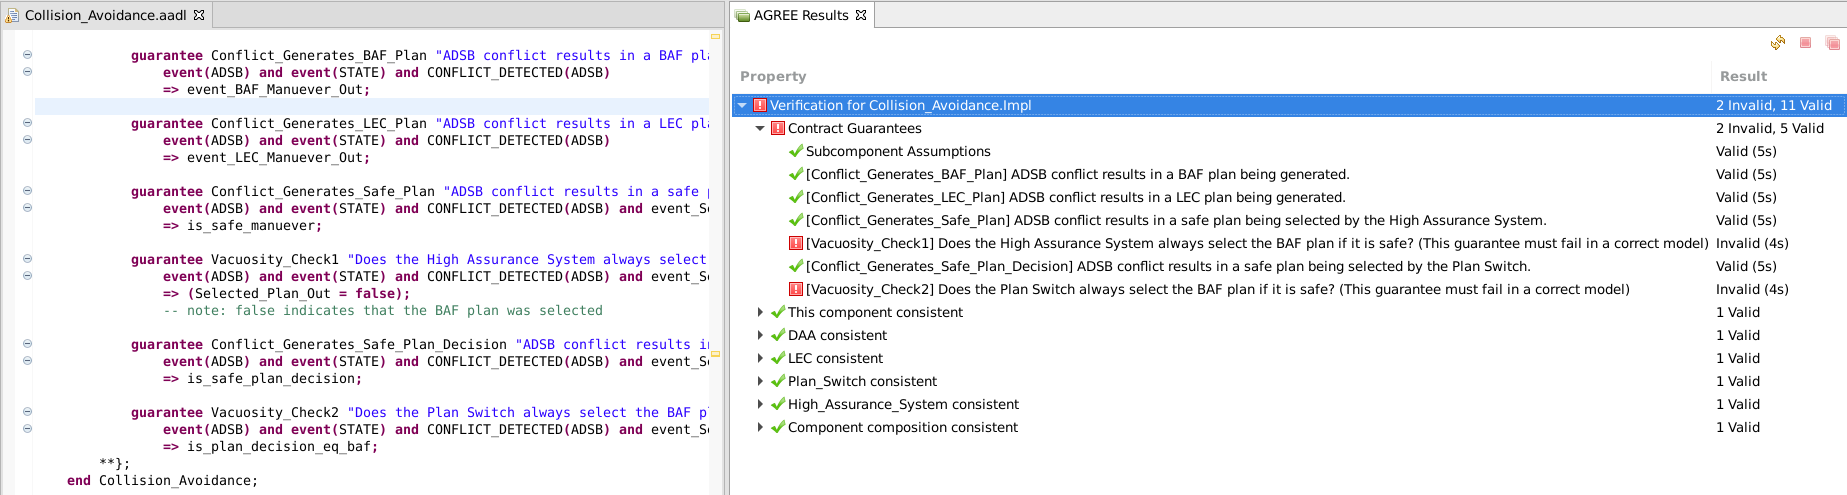
\includegraphics[width=\textwidth]{figures/rta-agree-v2.jpg}
	\caption{AADL Model of Run-Time Assurance Architecture and AGREE properties}
	\label{fig:rta-agree}
\end{figure*}
